% !TEX program = xelatex

\documentclass{beamer}
\usetheme{default}

\usepackage{ctex}

\title{Blockchain at the Edge: Performance of Resource-Constrained IoT Networks}
\author{张展鹏}
\begin{document}
\begin{frame}[plain]
    \maketitle
\end{frame}

\begin{frame}{物联网安全现状}
	器件差异性、局限性和传统安全方法面临的困难
	\begin{itemize}
		\item 物联网设备是海量的,设备间差异非常大,大部分是边缘设备;
		\item 边缘设备任务简单,专注于完成特定的简单任务和低功耗网络连接,几乎无多余的资源承载额外的安全机制;
		\item 物联网设备自身存在系统性和习惯性安全缺陷,例如弱密码、硬编码(固定)固码、缺乏安全访问的接口、不安全的数据访问和传输机制等;
		\item 物联网设备海量且空间位置不确定,管理员很难查找被感染或恶意设备;
		\item 当前主流的物联网安全方案依赖于集中式物联网网关,它会管理它负责的范围内物联网设备,目前物联网边缘快速拓展,集中式网关在长期难以适应这样的发展趋势。
	\end{itemize}
\end{frame}

\begin{frame}{物联网的“两域”和“六层”}
	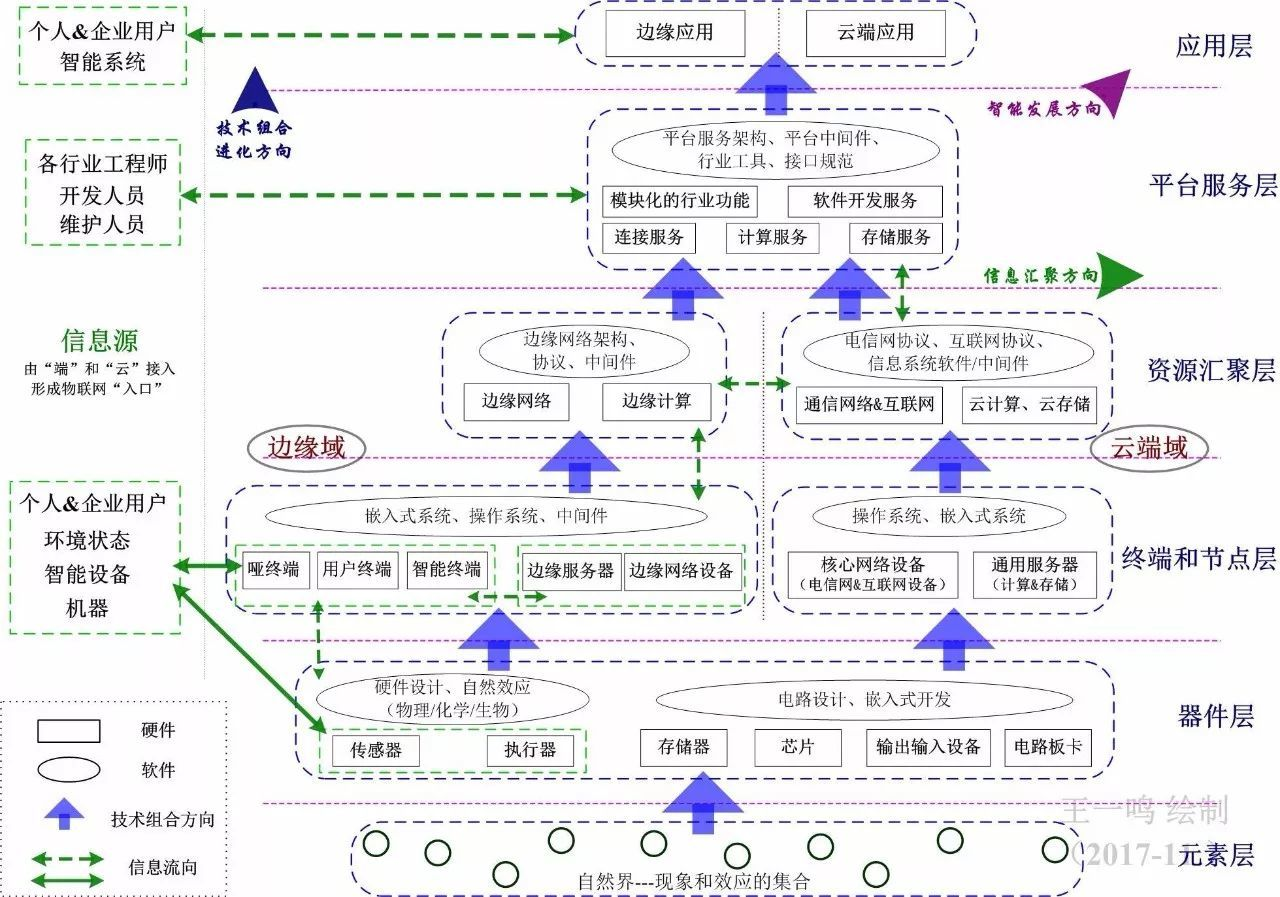
\includegraphics[width=\linewidth]{Assets/v2-7855b4b4d5101e18dc398cb0ca92d141_1440w}
\end{frame}

\begin{frame}{总体思路:从集中式到分布式}
	集中式网关的缺陷和分布式解决方案
	\begin{itemize}
		\item 集中式网关 v.s. 分布式网关
		\begin{itemize}
			\item 集中式网关位于资源汇聚层,由指定设备完成协议转换和流量转发,适合简单的一对多;集中式网关决定了它管理的全体设备的MAC地址,这意味着集中式网关的可拓展性差;
			\item 分布式网关位于终端和节点层,数量多、适合自动化部署、配置灵活、扩展性良好,分布式网关的流量转发路径最优。
		\end{itemize}
		\item 集中式网关不适合物联网,它无法阻止未经授权直接访问物联网边缘的行为,集中式网关依赖远程托管的安全机制,必然依赖云端管理者和集中式网关。
		\item 分布式系统的拓展性决定了它更适合作为物联网安全解决方案。区块链是典型的安全的分布式系统,链上数据不可篡改——区块链+物联网。
	\end{itemize}
\end{frame}

\begin{frame}{区块链应用在物联网的挑战}
	运算能力和网络状况
	\begin{itemize}
		\item 物联网设备越多,链上节点越多,每个链上节点,即物联网设备的运算和存储压力越大,物联网边缘设备不是为执行大量运算设计的,也不全有存储设备;
		\item 物联网设备的网络连接是受限的,链上节点必须同步数据,大多数物联网边缘设备无内部时钟,这类非实时性设备很难进行主动同步。
	\end{itemize}
\end{frame}

\begin{frame}{论文的模拟和解决方法}
	论文工作在4节点以太坊区块链展开,针对在运算能力和网络状况遇到的问题分别进行了模拟和解决。
	\begin{itemize}
		\item 为了模拟设备多样性和网络多样性,4个节点包括了以太网和我Wi-Fi连接的工作站和树莓派;
		\item 作者提出了一种可以应用在区块链中的中心化时间同步机制,通过传统的授时方案实现无内部时钟设备的时间设置和同步,这样的时间字符串是密文传输的。
	\end{itemize}
\end{frame}
\end{document}